\subsubsection{Estabilidad de GeM}
\label{subsec:exp7}
\begin{LaTeXdescription}
    \item[Objetivo] Observar el ranking de PageRank/GeM puede sufrir variaciones
        importantes de una fecha a la otra, al recibir un set nuevo de
        informaci\'on.\\

    \item[Hip\'otesis] GeM es m\'as inestable que la puntuaci\'on oficial del
        f\'utbol.\\

    \item[Proposici\'on] Nos interesa considerar casos extremos para evaluar la
        estabilidad del ranking que devuelve GeM. El sistema de puntaje actual
        del f\'utbol tiene la caracter\'istica de ser bastante ''estable'': en
        una \'unica fecha un equipo puede ganar a lo sumo 3 puntos, lo cual
        (salvo en los comienzos de un torneo o casos de empate m\'ultiple
        dif\'iciles de encontrar en la realidad) no lo hace avanzar m\'as de 4 o
        5 posiciones.

        \par Nos interesa analizar si esta propiedad se conserva en GeM. Para
        eso, imaginemos un torneo de f\'utbol desbalanceado, es decir, un torneo
        en que al finalizar, el primer equipo tiene mucha diferencia con el
        \'ultimo\footnote{Consideramos esto desbalanceado. Si no es este el
        caso del lector, simplemente considerar una instancia que cumpla con esa
        condici\'on.}. Si en una \'ultima fecha ''inventada'', agregada
        artificialmente, el \'ultimo le ganase al primero, el m\'etodo de
        puntuaci\'on est\'andar dif\'icilmente altere demasiado el ranking.
        Queremos observar si esto ocurre con GeM.\\

    \item[M\'etodo de Experimentaci\'on] Tomamos el Campeonato de Primera B
        Nacional 2013/14, en el cual Banfield (1º) termin\'o con 78 puntos
        mientras que Villa San Carlos (22º y \'ultimo) termin\'o con 24.
        Generamos una fecha artificial extra en la que Villa San Carlos le gana
        a Banfield. El ranking oficial no cambiar\'ia, dado que con 27
        puntos Villa San Carlos seguir\'ia \'ultimo. De confirmarse nuestra
        hip\'otesis, esperar\'iamos ver un cambio en la posición que GeM le
        asigna a Villa San Carlos. En este caso, variando la cantidad de goles,
        estudiamos cu\'anto se alterar\'ia el resultado si la victoria fuese
        m\'as abultada. El valor de $\alpha$ usado fue de 0.85.\\

    \item[Resultados, an\'alisis y discusi\'on]
\end{LaTeXdescription}

\par Se confirmó la hipótesis. Efectivamente GeM altera el ranking por una
simple victoria por 1 a 0, aunque Villa San Carlos sigue último. Esto se debe a
que el puntaje GeM de Banfield cae y el de VSC sube, alterando a los demás
equipos que ganaron o perdieron contra alguno de ellos.

\begin{figure}[H]
    \caption{Consecuencias de introducir un partido artificial}
    \centering
    \subfloat[][Distancia GeM Adulterado vs Oficial/GeM\label{subfig:exp7_dist_ranks}]{
        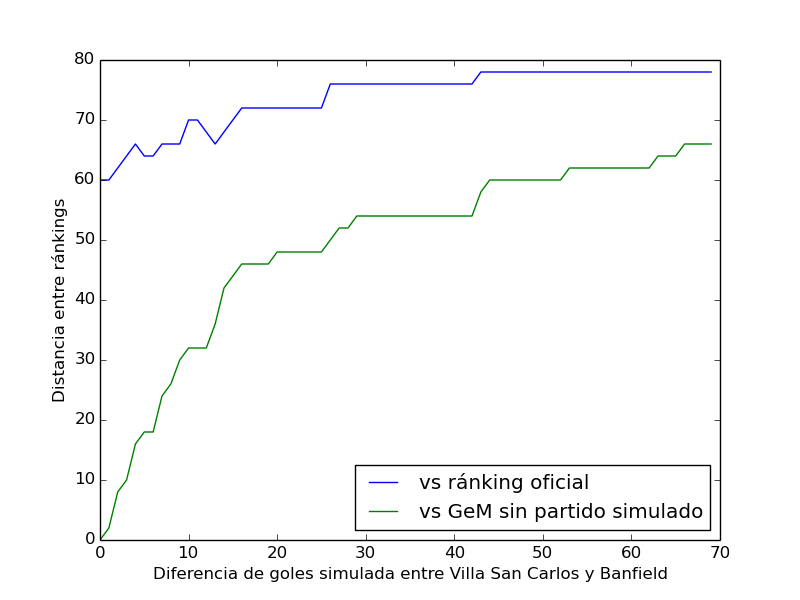
\includegraphics[width=.45\textwidth]{exp7_diferencia_ranks_funcion_goles.png}
    }\hspace{2pt}
    \subfloat[][Posición de Villa San Carlos en GeM Adulterado\label{subfig:exp7_pos_vsc}]{
        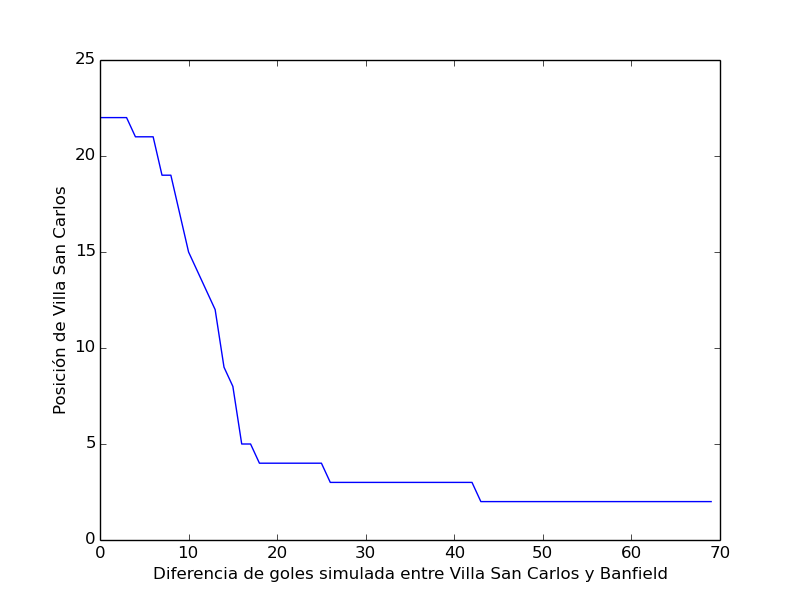
\includegraphics[width=.45\textwidth]{exp7_poscion_villa_san_carlos.png}
    }
\end{figure}

\par Alcanza con una victoria de 4 a 0 para que Villa San Carlos deje el último
lugar. Y con una victoria de 43 a 0 pasa a estar en 2do lugar. Si esto parece
irreal, considerar el récord del fútbol profesional de goles en un mismo
partido: \emph{AS Adema 149 - 0 SO l'Emyrne}, el 31 de octubre de 2002 por la
\emph{THB Champions League de Madagascar}\footnote{En honor a la verdad, este
resultado fue alcanzado por goles en contra por protesta contra el arbitraje.
El resultado ``honesto'' más abultado fue \emph{Arbroath FC 36 - 0 Bon Accord
FC}, el 12 de septiembre de 1885 por la Copa Escocesa 1885-86 y, más
recientemente, el conocido \emph{Australia 31 - 0 Samoa Americana}, el 11 de
abril de 2001, por la clasificación al Mundial de Fúbol Corea-Japón 2002}.

\par En la figura \ref{subfig:exp7_pos_vsc} se puede observar la posición de
Villa San Carlos en función de la cantidad de goles del partido artificial. En
la figura \ref{subfig:exp7_dist_ranks} se puede observar la diferencia entre
rankings producida por el partido simulado en función de la cantidad de goles
del partido. Se observa claramente la ``inestabilidad'' de la que hablábamos:
por los resultados de un simple partido GeM puede alterar el orden en un factor
grande. Consideramos que esta no es una propiedad deseable del sistema, al
menos no para el fútbol: hay muchos factores que influyen en un resultado,
independientemente de la calidad de los competidores (azar, arbitraje, clima,
estado del campo, etc.). Un equipo ``malo'' no debería dejar de serlo solo por
haber haber tenido suerte (o incluso por haber hecho un único buen partido)
contra un equipo ``bueno'', o porque su rival haya hecho un partido malo.

\par El próximo experimento apunta a dejar aún más en evidencia esta situación.
